\documentclass[../main.tex]{subfiles}

\begin{document}

This chapter gives a sketch of the inner structure of clauses.
Most of the time it is about simple clauses\index{clause!simple} and leave subordination to 
\prettyref{chap:relative} and \prettyref{chap:comp-clause}.
This being said, matrix clauses\index{clause!matrix} (the surrounding environment of subordinated clauses)
will also appear briefly in this part, so what we are talking about in this chapter -- and this part -- is 
actually the $v$P layer and the TP layer, but not the CP layer, so topicalization etc. are not 
discussed in this part. 

We can further break the $v$P layer -- 
in more descriptive terms, the argument structure\index{argument structure}, associated motions, etc.
-- from the TP layer -- 
in more generative terms, marking of the manner, time, etc. of an event and the obligatory topic. 
There are descriptive works organizing chapters about clause structure in this way, 
example \citet{jacques2021grammar} for Japhug, 
in which \citechap{14} and \citechap{15} discuss the argument structure 
and associated motions (unmarked $v$P properties), 
and \citechap{17} to \citechap{19} discuss valency changing devices (valency changing $v$Ps), 
and \citechap{21} and \citechap{22} discuss TP properties of simple clauses. 
But doing so inevitably faces the barrier in \prettyref{sec:movement-in-theory}: 
it has to involve some kind of Spec-$v$P-to-Spec-TP A-movement, 
which is of course to be rejected in a descriptive grammar. 
\citet{jacques2021grammar} is able to doing so 
because Japhug has a complicated argument indexation system 
and therefore describing the argument structure out of the context of clausal structure (\citechap{14}) 
is acceptable for everyone.
On the other hand, Chinese does not have argument indexation and hence 
the argument structure itself may be considered as purely semantic by descriptive linguists
and does not worth a single chapter.

\section{Constituent order and partition}\label{sec:clause-constituent-order-overview}

\subsection{The School Grammar partition}

The School Grammar segments clausal constituents in a way quite similar to the \ac{cgel} approach. 
Take the analysis in a prevalent textbook \citet[\citechap{5}]{xianhan2004} as an example.
A clause is first divided into 主语 (subject) and 谓语, and 谓语 is then divided into 述语, 宾语 (object) and 补语,
and 谓语 has modifiers named 状语, while modifiers in NPs are named as 定语. We can almost identify 
谓语 as \emph{predicate}\index{predicate} in \ac{cgel}, and 述语 as \emph{predicator}\index{predicator}. 
The term for 状语 in \ac{cgel} is certainly \emph{adjunct}, but to avoid confusion we use \emph{adverbial}
here, in accordance with most works in Chinese grammar. 
Besides the subject-predicate construction 主谓结构, 
there are \ac{sfp} added to the whole clause, 
which, in the School Grammar, are often referred as 语气词 (lit. `speech tone word').
The School Grammar analysis of clause structure is thus 
be summarized as \prettyref{fig:school-grammar-clause}.
Note that the constituent order of the verb, 
the object(s) and non-argument complements are missing in the diagram, because 
the inner organization of the nucleus predicate is highly complicated and there is no universal scheme.
Note that in \prettyref{fig:school-grammar-clause},
there are % TODO: 我想说的是,[把A]打了和把[A打了]的分析似乎都站得住脚,所以此处不详细说明怎么做branching

\begin{figure}
    \centering
    

\tikzset{every picture/.style={line width=0.3pt}} %set default line width to 0.75pt        

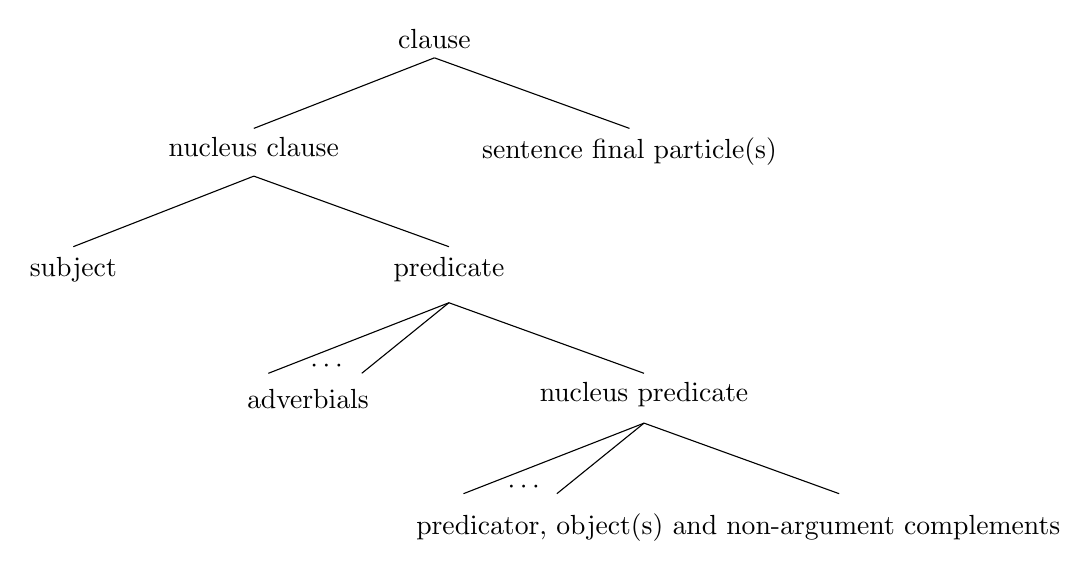
\begin{tikzpicture}[x=0.75pt,y=0.75pt,yscale=-1,xscale=1]
%uncomment if require: \path (0,383); %set diagram left start at 0, and has height of 383

%Straight Lines [id:da03870203201071365] 
\draw    (306,64.48) -- (219,98.48) ;
%Straight Lines [id:da09410121434078333] 
\draw    (306,64.48) -- (400,98.48) ;
%Straight Lines [id:da6473752338850502] 
\draw    (219,121.48) -- (132,155.48) ;
%Straight Lines [id:da22452164165522825] 
\draw    (219,121.48) -- (313,155.48) ;
%Straight Lines [id:da12042747516750363] 
\draw    (313,182.48) -- (226,216.48) ;
%Straight Lines [id:da6837235841990796] 
\draw    (313,182.48) -- (407,216.48) ;
%Straight Lines [id:da3234320748825805] 
\draw    (313,182.48) -- (271,216.48) ;
%Straight Lines [id:da4586272779304892] 
\draw    (407,240.48) -- (320,274.48) ;
%Straight Lines [id:da815197318792398] 
\draw    (407,240.48) -- (501,274.48) ;
%Straight Lines [id:da0031789117644716036] 
\draw    (407,240.48) -- (365,274.48) ;

% Text Node
\draw (306,61.48) node [anchor=south] [inner sep=0.75pt]   [align=left] {clause};
% Text Node
\draw (400,101.48) node [anchor=north] [inner sep=0.75pt]   [align=left] {sentence final particle(s)};
% Text Node
\draw (219,101.48) node [anchor=north] [inner sep=0.75pt]   [align=left] {nucleus clause};
% Text Node
\draw (132,159.48) node [anchor=north] [inner sep=0.75pt]   [align=left] {subject};
% Text Node
\draw (313,159.48) node [anchor=north] [inner sep=0.75pt]   [align=left] {predicate};
% Text Node
\draw (245,209) node [anchor=north west][inner sep=0.75pt]   [align=left] {$\displaystyle \cdots $};
% Text Node
\draw (207,223) node [anchor=north west][inner sep=0.75pt]   [align=left] {\begin{minipage}[lt]{55.17pt}\setlength\topsep{0pt}
\begin{center}
adverbials
\end{center}

\end{minipage}};
% Text Node
\draw (407,219.48) node [anchor=north] [inner sep=0.75pt]   [align=left] {nucleus predicate};
% Text Node
\draw (340,267) node [anchor=north west][inner sep=0.75pt]   [align=left] {$\displaystyle \cdots $};
% Text Node
\draw (296,283) node [anchor=north west][inner sep=0.75pt]   [align=left] {predicator, object(s) and non-argument complements};


\end{tikzpicture}

    \caption{The School Grammar analysis of clause structure}
    \label{fig:school-grammar-clause}
\end{figure}

This top-down analysis is 
also the starting point of this book's discussion of clause structure. 
% TODO: 展示各章节之间的联系

\subsection{Distribution of lexical categories in the clause level}

\prettyref{fig:school-grammar-clause} is more about syntactic functions than the inner structure of constituents.
The prototypical contents of argument positions are of course NPs, 
while the predicator is prototypically filled by a verb 
(and the nucleus predicate is the verb phrase headed by the verb), 
but things may vary.
Chinese does not have a morphological complementation device,
be it nominalization, gerund or infinitive, 
so verb phrases can fill argument positions, too, 
just like how nominalized verbs or complement clauses fill argument positions 
in languages with richer morphology. % TODO: link
Consider, for example:
\begin{exe}
    \ex \gll [ 算 费曼-图 ]_{\text{verb phrase}} 是 非常 费力 的 。\\
    {} calculate Feynman-diagram {} is very consume-power DE \\ % TODO: glossing
    \glt `[Calculating Feynman diagrams] is very exhausting.'
\end{exe}
We do not need to apply any morphological marking on the verb 算, which heads the subject.

Besides verbs, adjectives can fill the predicator position and other predicative positions, too.  % TODO: link

\subsection{The position of sentence final particles}

There are some disagreements about the position of \ac{sfp}s. 
Some place them into the predicate \citep[\citesec{16.1.1}]{zhudexigrammar}. 
The disputation here is just like the disputation about whether the object is a part of the verb phrase 
(\prettyref{sec:divergent-standard-constituency-segmentation}).
The \ac{sfp}s are in the CP layer, and the definition of the predicate is somehow unclear.
If we define it as ``what remains in the TP layer after removing the subject'',
then the \ac{sfp} is not in the predicate for obvious reasons.
Under this definition, \prettyref{fig:school-grammar-clause} makes perfect sense.
If, however, we define the predicate as 
``the main verb and all dependents of the verb that are not topic-like'',
then \ac{sfp}s should be included into the predicate.
From a generative perspective, the second definition is not natural enough,
because this means the coarse-grained tree undergoes a not-so-local reconstruction: 
something in the CP layer is inserted into the TP layers below the subject,
and it is highly unlikely to see a grammar construction work on this definition of \term{predicate}.

\section{The nucleus predicate}

% TODO:句子中的全局依赖全部放到这里: 一个construction作为另一个construction的输入

There are several grammatical systems in the nucleus predicate, including 
the direct and indirect objects (\prettyref{chap:subject-object}),
the non-argument complement construction (\prettyref{chap:non-argument-complement}),
the serial verb construction (\prettyref{chap:serial-verb-construction}),
the aspectual system(s) (\prettyref{chap:aspect}),
and the polarity (\prettyref{chap:negation}). 
These systems are not orthogonal. 
Polarity marking is related to the kind of complement in the predicate:
the negative form of a potential complement construction cannot be obtained by simply adding a negative operator 
(\prettyref{sec:direction-potential-complement}, ). % TODO: 可能补语的否定形式
The ``weight'' of the direction complement is related to the relative order 
between the direction complement and the aspectual marker. % TODO: 走了上去
Finally, the function of the subject is related to the function of the predicate,
and hence strongly influences the structure of the nucleus predicate. 
% TODO: 列出各个构式施加的顺序

The behaviors of these systems are important criteria of verb classes. % TODO: 动词分类

In the post-verbal position are 
aspectual suffixes (\prettyref{sec:post-verbal-aspect}),
direction complements(\prettyref{sec:direction-complement}), % TODO: 更全面的列表
The constituent order in the nucleus predicate is the follows:
\begin{exe}
    \ex 
\end{exe}

\subsection{Negation}

There is no negative concord in Chinese, 
but there is no uniform negation operator like the English \emph{not} in Chinese, either. 

The closest thing to the English \emph{not} is 不. 
Verbs can be negated by 不 while nouns generally cannot, 
and this is a criterion to tell verbs from nouns. 
Other negation operators and strategies are used frequently.
The negation operator 没 is used to negate , V不了, 
% TODO: 决定是否单独开一章写否定;以及这一节怎么整理

\begin{exe}
    \ex \begin{xlist}
        \ex 我做 [不了]_{\text{potential complement, negative}} 这件事。
        \ex[*]{我\{没有/并非/不\}_{\text{negative operator}} 做 [得了]_{\text{potential complement, positive}} 这件事。}
    \end{xlist}    
\end{exe}


\end{document}